%%%%%%%%%%%%%%%%%%%%%%%%%%%%%%%%%%%%%%%%%%%%%%%%%%%%%%%%%%%%%%%%%%%%%%%%%%%%%
%% Descr:       Vorlage für Berichte der DHBW-Karlsruhe, Ein Kapitel
%% Author:      Prof. Dr. Jürgen Vollmer, vollmer@dhbw-karlsruhe.de
%% $Id: kapitel2.tex,v 1.5 2017/10/06 14:02:51 vollmer Exp $
%%  -*- coding: utf-8 -*-
%%%%%%%%%%%%%%%%%%%%%%%%%%%%%%%%%%%%%%%%%%%%%%%%%%%%%%%%%%%%%%%%%%%%%%%%%%%%%%%



\chapter{Grundlagen}
In diesem Kapitel werden die Grundlagen der verwendeten Werkzeuge sowie die theoretischen Grundladen erläutert.
\section{React}
In diesem Unterkapitel werden die Grundlagen von React näher beschrieben um ein grundlegendes Verständnis zu generieren.

1.2 Überblick über React
React ist eine populäre JavaScript-Bibliothek zur Erstellung von Benutzeroberflächen und bietet zahlreiche Vorteile für Entwickler. Um React effektiv nutzen zu können, wird empfohlen, fundierte JavaScript-Kenntnisse zu haben[1].

Einige der Hauptmerkmale von React sind:

Komponentenbasierte Architektur: React verwendet eine komponentenbasierte Architektur, die die Entwicklung modularer und wiederverwendbarer Benutzeroberflächen ermöglicht. Jede Komponente in React ist verantwortlich für einen bestimmten Teil der Benutzeroberfläche und kann unabhängig von den anderen Komponenten aktualisiert und gewartet werden.

Einweg-Datenfluss: React verwendet einen einseitigen Datenfluss, der auch als "unidirektionaler Datenfluss" bezeichnet wird. Dies bedeutet, dass die Daten in einer React-Anwendung in einer einzigen Richtung fließen, was die Komplexität der Anwendung reduziert und die Vorhersagbarkeit des Verhaltens der Anwendung verbessert.

Virtuelles DOM: React verwendet ein virtuelles DOM (Document Object Model), um Änderungen an der Benutzeroberfläche effizient zu verwalten. Das virtuelle DOM ist eine leichtgewichtige In-Memory-Repräsentation des tatsächlichen DOM und ermöglicht es React, Änderungen an der Benutzeroberfläche schnell zu berechnen und nur die tatsächlich geänderten Teile des DOM zu aktualisieren. Dies führt zu einer schnelleren Leistung und einer besseren Benutzererfahrung.

Insgesamt bietet React eine leistungsstarke und flexible Lösung für die Erstellung von modernen Benutzeroberflächen und Webanwendungen, die leicht zu entwickeln, zu warten und zu skalieren sind
\subsection{Hintergrund und Motivation}
React ist eine JavaScript-Bibliothek zur Erstellung von Benutzeroberflächen, die von Facebook entwickelt wurde und seit 2013 öffentlich verfügbar ist.\cite{ReactGettingStarted} Die Hauptmotivation für die Entwicklung von React bestand darin, die Leistung und Skalierbarkeit von Facebooks eigenen Webanwendungen zu verbessern. Insbesondere suchten die Facebook-Entwickler nach einer Möglichkeit, große und komplexe Anwendungen zu erstellen, die schnell, reaktionsfreudig und einfach zu warten sind. React ermöglicht es Entwicklern, wiederverwendbare Komponenten zu erstellen, die einfach zu pflegen und zu aktualisieren sind. Darüber hinaus kann React für verschiedene Anwendungen eingesetzt werden, einschließlich Single-Page-Anwendungen, Mobile-Apps und serverseitige Anwendungen.

\begin{figure}[htbp]
	\centering
	\fbox{
\includegraphics[height=0.3\textheight]{images/react-logo}}
	\caption{React-Logo}
\end{figure}

\subsection{Überblick über React}

React ist eine bekannte JavaScript-Bibliothek, die zur Erstellung von Benutzeroberflächen verwendet wird und auf einem komponentenbasierten Ansatz basiert. Laut der offiziellen React-Dokumentation ermöglicht React eine deklarative Syntax, um UI-Komponenten zu definieren und zu rendern, die wiederverwendet werden können, um komplexe Benutzeroberflächen zu erstellen.\cite{ReactJS} 

Es gibt mehrere Gründe, warum es sinnvoll ist, React zu erlernen. Ein wichtiger Grund ist, dass React auf JavaScript basiert und Entwicklern, die bereits JavaScript beherrschen, den Einstieg erleichtert. Ein weiterer Vorteil ist, dass React auf einem komponentenbasierten Ansatz basiert, der es einfacher macht, Webanwendungen in kleine, wiederverwendbare Komponenten aufzuteilen, die unabhängig voneinander erstellt und gewartet werden können.\cite{Kinsta} 

Eine weitere Stärke von React ist die effektive Verwaltung des Zustands und die leistungsstarke Wiederverwendbarkeit von Komponenten. Dadurch wird die Entwicklung von Webanwendungen beschleunigt. Zudem gibt es eine engagierte Entwicklergemeinschaft, die sich ständig weiterentwickelt und verbessert, was zu einer hohen Verfügbarkeit von Lernressourcen und ständigen Verbesserungen der Bibliothek führt.\cite{Kinsta}

Die Beliebtheit von React in der Entwicklergemeinschaft zeigt sich auch in der Stack Overflow Umfrage 2021, bei der React als eine der beliebtesten Technologien im Bereich der Web-Frameworks genannt wurde.\cite{StackOverflowSurvey}

React hat auch die Entwicklung von Single-Page-Applications vereinfacht, indem es eine schnelle und nahtlose Benutzererfahrung ermöglicht, ohne dass die Seite neu geladen werden muss.\cite{Kinsta}

Zusammenfassend ist React eine wertvolle Fähigkeit für Webentwickler, da es eine effektive Verwaltung des Zustands und eine leistungsstarke Wiederverwendbarkeit von Komponenten bietet und die Entwicklung von Single-Page-Applications vereinfacht. Die Beliebtheit von React in der Entwicklergemeinschaft unterstreicht zudem seine Bedeutung für die Webentwicklung.

\subsection{Grundlagen über React}
\subsubsection{Virtual DOM}
Das Virtual DOM ist ein zentrales Konzept von React, einer JavaScript-Programmbibliothek zur Erstellung von webbasierten Benutzeroberflächen\cite{ReactWikipedia}. Es handelt sich dabei um eine leichtgewichtige JavaScript-Darstellung des Document Object Model (DOM), die in deklarativen Web-Frameworks wie React, Vue.js und Elm verwendet wird \cite{VueJsAdesso}. Das Virtual DOM ermöglicht es React, minimale DOM-Operationen auszuführen, wenn die Benutzeroberfläche neu gerendert wird. Im Gegensatz zum tatsächlichen DOM ist das Virtual DOM eine Art abstrakte Kopie, die deutlich kleiner ist und auf das Nötigste an Informationen beschränkt.\cite{ReactWikipedia}

Das Virtual DOM bietet mehrere Vorteile für die Entwicklung von Webanwendungen. Zum einen abstrahiert es manuelle DOM-Manipulationen vom Entwickler, was die Entwicklung von komplexen Benutzeroberflächen vereinfacht und zu einem vorhersehbareren Verhalten der Anwendung führt [1]. Zum anderen ermöglicht das Virtual DOM inkrementelles Rendering, was bedeutet, dass React nur die Komponenten rendert, die sich tatsächlich geändert haben \cite{ReactWikipedia}. Dies führt zu einer effizienteren Ausführung von Benutzeroberflächen-Updates und einer insgesamt schnelleren Anwendung.

Das folgende Bild illustriert den Unterschied zwischen dem tatsächlichen DOM und dem Virtual DOM:


\begin{figure}[htbp]
	\centering
	\fbox{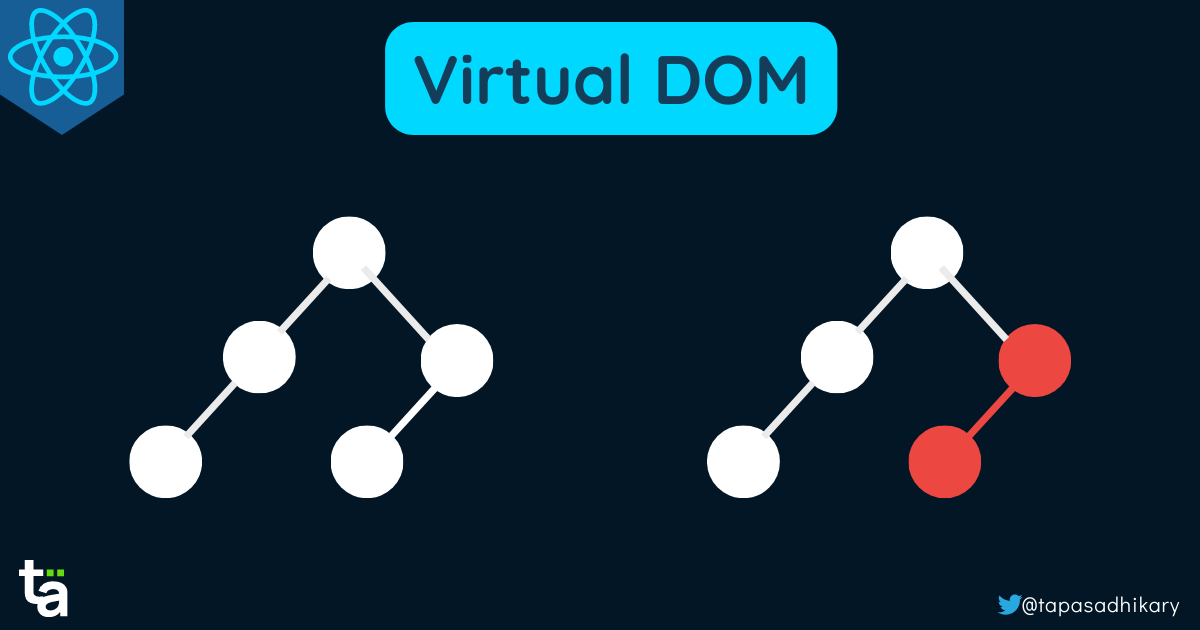
\includegraphics[height=0.3\textheight]{images/virtualDom}}
	\caption{Virtual-DOM}
\end{figure}
Das Bild zeigt schematisch, wie das Virtual DOM in React funktioniert. Zunächst wird eine virtuelle Darstellung des DOMs in Form eines Baumes erstellt. Bei Änderungen an der Benutzeroberfläche wird ein neuer Baum erstellt und mit dem vorherigen Baum verglichen. Dabei werden nur die Unterschiede zwischen den beiden Bäumen ermittelt. Anschließend werden nur die geänderten Elemente im tatsächlichen DOM aktualisiert. Dieser Prozess wird als Reconciliation bezeichnet \cite{ReactVirtualDOM}.

\subsubsection{Komponenten und Props}
React ist eine Bibliothek für die Entwicklung von Benutzeroberflächen, die auf dem Konzept von Komponenten und Props basiert. Eine React-Komponente ist eine eigenständige und wiederverwendbare Einheit einer Benutzeroberfläche, die entweder als Klasse oder als Funktion definiert werden kann. Komponenten können andere Komponenten enthalten und selbst als Teil einer größeren Anwendung verwendet werden \cite{ReactComponentsAndProps}.

Props (kurz für "Properties") sind ein wichtiger Mechanismus zur Konfiguration von React-Komponenten. Sie dienen zum Übergeben von Daten von einer Komponente zur anderen und werden als Objekt an die Komponente übergeben. Innerhalb der Komponente können Props als Parameter verwendet werden. Im Gegensatz zum State, der zur Änderung der Benutzeroberfläche innerhalb einer Komponente verwendet wird, sind Props schreibgeschützt und können nicht direkt geändert werden. Durch das Verwenden von Props können Komponenten einfach wiederverwendet werden, indem sie in verschiedenen Kontexten mit unterschiedlichen Props konfiguriert werden \cite{ReactComponentsAndProps}.

Ein Beispiel für eine React-Komponente mit Props ist die Funktion \verb|Greeting|, die einen Gruß mit dem Namen des Benutzers anzeigt. Der Name wird als Prop an die Komponente übergeben und innerhalb der Funktion als Parameter verwendet. Hier ist das Codebeispiel:

\begin{verbatim}
	import React from 'react';
	
	function Greeting(props) {
		return <h1>Hello, {props.name}!</h1>;
	}
	
	export default Greeting;
\end{verbatim}

Alle React-Komponenten müssen sich im Bezug auf ihre Props als sogenannte "pure functions" verhalten \cite{ReactComponentsAndProps}. Das bedeutet, dass die Funktion der Komponente nur von ihren Props abhängen sollte und keine weiteren Seiteneffekte haben darf. Eine Komponente, die sich wie eine "pure function" verhält, ist leichter zu testen und zu warten.

Es gibt auch fortgeschrittene Konzepte im Zusammenhang mit Props, wie das Konzept des "Render Props". Hierbei handelt es sich um eine Technik zum Austauschen von Code zwischen React-Komponenten, bei der eine Komponente eine Funktion als Prop akzeptiert, die ein React-Element zurückgibt. Dadurch können Komponenten dynamisch wiederverwendet werden und die Codebasis der Anwendung wird vereinfacht\cite{ReactRenderProps}.

Um mit React-Komponenten und Props zu arbeiten, gibt es verschiedene Möglichkeiten. Funktionskomponenten sind die einfachste Art, eine Komponente zu definieren, indem man eine JavaScript-Funktion schreibt. Klassenkomponenten bieten mehr Funktionen, wie den Zugriff auf den State, die Möglichkeit, Lifecycle-Methoden zu definieren und vieles mehr \cite{RunebookReactComponentsAndProps}.

Insgesamt sind Komponenten und Props wichtige Konzepte in React, die Entwicklern helfen, wiederverwendbare Benutzeroberflächenkomponenten zu erstellen und die Effizienz der Entwicklung zu erhöhen. Durch das Verwenden von
\subsubsection{State}
In React ist der "State" ein Objekt, das in einer Komponente definiert wird und Werte speichert, die zur Laufzeit der Anwendung verändert werden können. Der Zustand wird in der Regel verwendet, um die Darstellung der Benutzeroberfläche zu aktualisieren, wenn sich etwas ändert. Wenn der Zustand eines Komponentenobjekts geändert wird, wird die Methode "render()" aufgerufen, um die Änderungen in der Benutzeroberfläche anzuzeigen \cite{W3SchoolsReactState}.

Der Zustand wird oft als Schlüssel-Wert-Paar-Objekt definiert, wobei jeder Schlüssel eine Eigenschaft repräsentiert, die geändert werden kann, und jeder Wert den aktuellen Wert dieser Eigenschaft darstellt. State-Objekte können als eine Art Konfiguration betrachtet werden, die der Komponente zur Verfügung gestellt werden, um ihre Eigenschaften und ihr Verhalten zu steuern \cite{FreeCodeCampStateInReact}.

Der Zustand ist ein Beobachtbares Objekt und kann somit verändert werden. In React-Komponenten kann der Zustand durch die Verwendung der "setState()" Funktion aktualisiert werden.

Eine sorgfältige Verwaltung des Zustands in einer React-Anwendung ist wichtig, um Fehler zu vermeiden und die Leistung zu optimieren. Die Organisation des Zustands und die Datenfluss zwischen den Komponenten sollten gut durchdacht sein, um überflüssigen oder doppelten Zustand zu vermeiden \cite{ReactManagingState}.

Hier ist ein Beispiel, das zeigt, wie der Zustand in React-Komponenten implementiert werden kann:

\begin{lstlisting}[language=vhdl,
	frame=single,           % Ein Rahmen um den Code
	framexleftmargin=15pt,  % Rahmen link von den Zahlen
	style=algoBericht,
	label={Dockerfile},
	captionpos=b           % Caption unter den Code setzen
	caption={.env für DHBW-Star}]
	import React, { useState } from "react";
	
	function Example() {
		// Initialisieren des State-Objekts
		const [count, setCount] = useState(0);
		
		Erhoehen des Zaehlers, wenn der Button geklickt wird
		function increaseCount() {
			setCount(count + 1);
		}
		
		return (
		<div>
		<p>You clicked {count} times</p>
		<button onClick={increaseCount}>Click me</button>
		</div>
		);
	}
\end{lslisting}

In diesem Beispiel wird die \emph{useState()} -Hook verwendet, um den Zustand der Komponente zu initialisieren. Die Funktion \emph{useState()} gibt ein Array zurück, das den aktuellen Zustand und eine Funktion zur Aktualisierung des Zustands enthält. In diesem Fall wird der Zustand mit \emph{count} initialisiert und die Funktion \emph{setCount()} wird verwendet, um den Zustand zu aktualisieren. Wenn der Button geklickt wird, wird die \emph{increaseCount()} Funktion aufgerufen, die den Zähler erhöht und den Zustand mithilfe von \emph{setCount()} aktualisiert. Die Änderung des Zustands löst eine erneute Ausführung der Komponente aus, und die aktualisierten Werte werden in der Benutzeroberfläche angezeigt.


\subsection{Verwendung von React}
\subsubsection{Einrichtung von React}
 React ist eine Bibliothek für JavaScript, die von Facebook entwickelt wurde und zur Erstellung von Benutzeroberflächen eingesetzt wird. Um React in einem Projekt verwenden zu können, muss es zuerst eingerichtet werden. Die offizielle Dokumentation von React bietet eine ausführliche Anleitung zur Einrichtung von React \cite{ReactDocsSetup}.

Eine Möglichkeit, React in einem neuen Projekt zu installieren, besteht darin, ein neues Projektverzeichnis zu erstellen und dann das React-Paket über NPM zu installieren:

\begin{verbatim}
	npx create-react-app my-app
	cd my-app
	npm start
\end{verbatim}

Dieser Befehl erstellt ein neues React-Projekt mit dem Namen "my-app" und startet den Entwicklungsserver.

Es ist auch möglich, React manuell in ein bestehendes Projekt einzubinden. In diesem Fall müssen die React- und React-DOM-Pakete installiert werden:

\begin{verbatim}
	npm install react react-dom
\end{verbatim}

Es gibt auch alternative Möglichkeiten, React in einem Projekt zu integrieren. Eine solche Möglichkeit ist die Verwendung von Create-React-App oder anderen Boilerplate-Vorlagen, die eine vorkonfigurierte React-Umgebung bereitstellen.
\subsubsection{Komponentenentwicklung}
In React werden UI-Elemente in Komponenten zerlegt. Eine Komponente kann entweder als Funktion oder als Klasse definiert werden. Eine Klasse-Komponente bietet zusätzliche Funktionen und Möglichkeiten, während Funktions-Komponenten eine einfachere Syntax haben.

Eine Beispielkomponente könnte wie folgt aussehen:

\begin{verbatim}
	import React from 'react';
	
	function Greeting(props) {
		return <h1>Hello, {props.name}!</h1>;
	}
	
	export default Greeting;
\end{verbatim}

Diese Komponente heißt "Greeting" und nimmt ein Objekt mit einem Namen als Prop entgegen. Wenn diese Komponente gerendert wird, wird sie "Hello, {props.name}!" als Überschrift ausgeben.

Es ist auch möglich, eine Komponente als Klasse zu definieren:

\begin{verbatim}
	import React, { Component } from 'react';
	
	class Greeting extends Component {
		render() {
			return <h1>Hello, {this.props.name}!</h1>;
		}
	}
	
	export default Greeting;
\end{verbatim}

Diese Klasse-Komponente heißt auch "Greeting" und nimmt ein Objekt mit einem Namen als Prop entgegen. Wenn diese Komponente gerendert wird, wird sie "Hello, {this.props.name}!" als Überschrift ausgeben.
\subsubsection{Ereignisbehandlung}
In React werden Ereignisse behandelt, indem man einem bestimmten UI-Element (z.B. einem Button oder einer Input-Box) eine Event-Handler-Funktion zuweist. Diese Funktion wird aufgerufen, wenn das Ereignis ausgelöst wird, z.B. wenn auf den Button geklickt wird.

Hier ist ein Beispiel einer Button-Komponente mit einem Event-Handler:

\begin{verbatim}
	import React from 'react';
	
	function Button(props) {
		function handleClick() {
			console.log('Button clicked');
		}
		
		return (
		<button onClick={handleClick}>
		{props.label}
		</button>
		);
	}
	
	export default Button;
\end{verbatim}

Diese Button-Komponente nimmt ein Label als Prop entgegen und weist dem Button-Element einen Event-Handler (handleClick) zu. Wenn der Button geklickt wird, wird die Funktion handleClick aufgerufen und 'Button clicked' wird in der Konsole ausgegeben.

Es ist auch möglich, den Event-Handler in einer Klasse-Komponente zu definieren:

\begin{verbatim}
	import React, { Component } from 'react';
	
	class Button extends Component {
		handleClick() {
			console.log('Button clicked');
		}
		
		render() {
			return (
			<button onClick={this.handleClick}>
			{this.props.label}
			</button>
			);
		}
	}
	
	export default Button;
\end{verbatim}

Diese Button-Komponente definiert den Event-Handler in der Klasse und verwendet die Syntax this.handleClick, um den Handler dem Button zuzuweisen.
\subsubsection{JSX}
JSX ist eine von React verwendete Syntax, die es ermöglicht, HTML-ähnlichen Code innerhalb von JavaScript zu schreiben. JSX wird während der Kompilierung in normales JavaScript umgewandelt, so dass es vom Browser verstanden werden kann.

Hier ist ein Beispiel einer JSX-Komponente:

\begin{verbatim}
	import React from 'react';
	
	function Greeting(props) {
		return <h1>Hello, {props.name}!</h1>;
	}
	
	export default Greeting;
\end{verbatim}

Diese Komponente verwendet JSX, um das HTML-ähnliche Element <h1>Hello, {props.name}!</h1> zurückzugeben. Die geschweiften Klammern {} werden verwendet, um JavaScript-Code innerhalb von JSX auszuführen.

Es ist auch möglich, JavaScript-Ausdrücke innerhalb von JSX zu verwenden, um dynamischen Inhalt zu erzeugen:

\begin{verbatim}
	import React from 'react';
	
	function Greeting(props) {
		const greeting = Hello, ${props.name}!;
		
		return <h1>{greeting}</h1>;
	}
	
	export default Greeting;
\end{verbatim}

In diesem Beispiel wird die JavaScript-Variablendeklaration const greeting verwendet, um den dynamischen Inhalt des Elements zu erzeugen.

\subsection{Fortgeschrittene Themen in React}
React bietet eine Vielzahl von fortgeschrittenen Techniken und Bibliotheken, um komplexe Anwendungen zu entwickeln. Einige dieser Techniken sind Redux oder Context API, React Router, React Hooks und serverseitiges Rendern.
\subsubsection{Redux oder Context API}
Redux und Context API sind zwei Bibliotheken für React, die es ermöglichen, Daten auf einfache Weise durch die Komponenten einer Anwendung zu verteilen. Redux ist ein leistungsfähiges Tool für die Verwaltung von Anwendungsdaten, während Context API eine leichtgewichtige Alternative ist \cite{reduxgettingstarted, reactcontext}.

Redux funktioniert auf der Grundlage eines zentralisierten Speichers, in dem alle Anwendungsdaten gespeichert werden. Jede Komponente, die Daten benötigt, kann sie einfach aus dem Store abrufen und bei Bedarf aktualisieren. Redux bietet auch Tools wie Actions, Reducers und Middleware, um die Verwaltung von Anwendungsdaten zu vereinfachen und zu automatisieren.

Context API hingegen ermöglicht es Entwicklern, Daten auf einfache Weise durch die Komponentenbaumhierarchie zu verteilen. Jede Komponente kann auf den Kontext zugreifen und Daten abrufen oder aktualisieren, ohne auf Props oder eine globale Store-Instanz angewiesen zu sein. Context API ist eine einfachere Alternative zu Redux, die sich besser für kleinere Anwendungen eignet.
\subsubsection{React Router}
React Router ist eine Bibliothek für React, die es ermöglicht, dynamische URLs in einer Single-Page-Anwendung zu verwenden. Mit React Router können Entwickler die Navigation innerhalb der Anwendung auf einfache Weise definieren und steuern, ohne dass die Seite neu geladen werden muss. Die Integration von React Router in eine Anwendung ist relativ einfach und erfordert nur wenige Schritte \cite{reactroutertutorial, reactrouteroverview}.

React Router bietet verschiedene Funktionen wie die Definition von Routen und Parametern, die Möglichkeit zur Integration von Serverseitigem Rendering und die Möglichkeit, mit anderen Bibliotheken wie Redux zu interagieren. React Router ist eine wichtige Bibliothek für React-Entwickler, da es die Navigation innerhalb der Anwendung vereinfacht und eine bessere Benutzererfahrung bietet.
\subsubsection{React Hooks}
React Hooks ist eine Funktion in React, die es Entwicklern ermöglicht, Zustände und Effekte in funktionellen Komponenten zu verwenden. Mit Hooks können Entwickler den Zustand in einer Komponente speichern, ohne eine Klasse erstellen zu müssen \cite{reacthooksintro, w3schoolsHooks}.

Hooks bieten eine Reihe von Funktionen wie useState, useEffect und useContext, um den Zustand und die Effekte innerhalb der Komponente zu verwalten. Sie ermöglichen auch die Verwendung von benutzerdefinierten Hooks, um spezifische Funktionalitäten in verschiedenen Komponenten zu nutzen.
\subsubsection{Serverseitiges Rendern}
Serverseitiges Rendern (SSR) ist ein Prozess, bei dem React-Komponenten auf dem Server gerendert werden, bevor sie an den Browser gesendet werden. SSR bietet viele Vorteile, darunter eine schnellere Ladezeit der Seite, bessere Suchmaschinenoptimierung und bessere Leistung auf langsamen oder mobilen Geräten \cite{reactssr1, reactssr2}.

SSR in React kann auf verschiedene Arten implementiert werden, je nach den Anforderungen der Anwendung. Die Integration von SSR erfordert jedoch in der Regel eine Reihe von Schritten, einschließlich der Konfiguration des Servers und der Anpassung der Anwendung.

\subsection{Best Practices in React-Entwicklung}
Modularität und Wiederverwendbarkeit von Komponenten ist ein wichtiger Aspekt bei der Entwicklung von React-Anwendungen. Durch die Aufteilung einer Anwendung in kleine, wiederverwendbare Komponenten kann der Code besser organisiert und leichter gewartet werden. Es ermöglicht auch die Erstellung von Komponenten-Bibliotheken, die in anderen Projekten wiederverwendet werden können \cite{dhiwise, reactcomponentlibrary}.

Um eine Komponente modular und wiederverwendbar zu gestalten, sollte sie unabhängig und gut dokumentiert sein. Die Komponente sollte spezifische Funktionen erfüllen und keine Abhängigkeiten von anderen Komponenten haben. Es ist auch wichtig, die Komponenten sauber zu benennen und ihre Funktionen klar zu dokumentieren.
\subsubsection{Testen von React-Anwendungen}
Das Testen von React-Anwendungen ist ein wichtiger Aspekt, um sicherzustellen, dass die Anwendung robust und fehlerfrei ist. Es gibt verschiedene Arten von Tests, die in React-Anwendungen durchgeführt werden können, wie Unit-Tests, Integrationstests und End-to-End-Tests \cite{reacttesting, reacthookstesting}.

Die Unit-Tests konzentrieren sich auf das Testen einer einzelnen Komponente, um sicherzustellen, dass sie wie erwartet funktioniert. Integrationstests testen die Interaktion zwischen verschiedenen Komponenten, während End-to-End-Tests die gesamte Anwendung testen.

Es ist wichtig, regelmäßig Tests durchzuführen und Testabdeckungen zu implementieren, um potenzielle Fehler zu identifizieren und zu beheben.
\subsubsection{Performance-Optimierung}
Performance-Optimierung ist ein wichtiger Aspekt bei der Entwicklung von React-Anwendungen, da eine schlechte Leistung zu einer negativen Benutzererfahrung führen kann. Es gibt verschiedene Möglichkeiten, die Performance von React-Anwendungen zu verbessern.

Eine Möglichkeit besteht darin, sicherzustellen, dass nur die notwendigen Komponenten gerendert werden. React bietet die Möglichkeit, Komponenten als pure Funktionen zu definieren, die nur von ihren Eingaben abhängen. Dadurch können unnötige Rendervorgänge vermieden werden.

Eine weitere Möglichkeit besteht darin, das Rendering von Komponenten zu optimieren. Eine Möglichkeit, dies zu tun, ist die Verwendung von Memoization. Memoization ist eine Technik, bei der das Ergebnis einer Funktion zwischengespeichert wird, wenn dieselben Eingaben erneut verwendet werden. Dadurch können unnötige Berechnungen vermieden werden.

Außerdem sollte darauf geachtet werden, dass Komponenten nicht zu viele Props erhalten, da dies die Leistung negativ beeinflussen kann. In diesem Fall sollte die Komponente möglicherweise in kleinere Komponenten aufgeteilt werden, die jeweils nur die notwendigen Props erhalten.

Eine weitere Möglichkeit, die Performance von React-Anwendungen zu verbessern, ist die Verwendung von Code-Splitting. Code-Splitting ist eine Technik, bei der der Code einer Anwendung in kleinere Stücke aufgeteilt wird, die separat geladen werden können. Dadurch kann die Ladezeit der Anwendung verringert werden (\cite{ReactOpt}, \cite{LogRocket}).
\subsubsection{Sicherheit und React}
Sicherheit ist ein wichtiger Aspekt bei der Entwicklung von React-Anwendungen, da Sicherheitslücken zu ernsthaften Problemen führen können. Es gibt verschiedene Best Practices, die bei der Entwicklung von sicheren React-Anwendungen beachtet werden sollten.

Eine Möglichkeit besteht darin, XSS-Angriffe (Cross-Site Scripting) zu vermeiden. XSS-Angriffe können dazu führen, dass schädlicher Code in die Anwendung eingeschleust wird. Um XSS-Angriffe zu vermeiden, sollten alle Daten, die von Benutzern eingegeben werden können, validiert und gefiltert werden. Darüber hinaus sollte auch das Rendering von HTML sorgfältig überwacht werden.

Eine weitere Möglichkeit, die Sicherheit von React-Anwendungen zu verbessern, besteht darin, die Codequalität zu verbessern. Eine gute Codequalität kann dazu beitragen, potenzielle Sicherheitslücken zu identifizieren und zu beheben, bevor sie ausgenutzt werden können.

Außerdem sollten bei der Entwicklung von React-Anwendungen Best Practices für die Sicherheit von Webanwendungen beachtet werden, wie z.B. die Verwendung von sicheren Passwörtern und die Vermeidung von unsicheren Bibliotheken oder Frameworks (\cite{ReactSecurity}, \cite{FreeCodeCamp}).

\subsection{Vergleich mit anderen Frontend-Technologien}
\subsubsection{Vor- und Nachteile von React im Vergleich zu Angular und Vue.js}
React, Angular und Vue.js sind beliebte Frontend-Technologien, die bei der Entwicklung von modernen Webanwendungen eingesetzt werden. Jede Technologie hat ihre Vor- und Nachteile, die bei der Wahl der Technologie berücksichtigt werden sollten.

React zeichnet sich durch seine Flexibilität und einfache Handhabung aus. Es ist eine Bibliothek und nicht ein vollständiges Framework, was bedeutet, dass Entwickler mehr Freiheit haben und nur die Teile von React verwenden können, die sie benötigen. Dadurch ist React auch in der Regel schneller und leichter als Frameworks wie Angular oder Vue.js. Außerdem ist React sehr beliebt und hat eine große und aktive Community, was zu einer Fülle von Ressourcen und Unterstützung führt (\cite{Hosttest}).

Im Vergleich zu Angular und Vue.js hat React jedoch auch einige Nachteile. Einer der Nachteile ist, dass React weniger Features und Werkzeuge bietet als Angular oder Vue.js. Dadurch müssen Entwickler möglicherweise zusätzliche Bibliotheken und Tools verwenden, um bestimmte Aufgaben zu erledigen. Ein weiterer Nachteil von React ist, dass es nicht so viele vorgefertigte UI-Komponenten wie Vue.js bietet, was die Entwicklung von Anwendungen erschweren kann (\cite{Kruschecompany}).
\subsubsection{Verwendung von React in größeren Projekten}
React eignet sich auch sehr gut für größere Projekte, da es die Möglichkeit bietet, Anwendungen in kleine, wiederverwendbare Komponenten aufzuteilen. Dadurch können Teams effizienter arbeiten und die Anwendung leichter warten und skalieren. Darüber hinaus bietet React auch die Möglichkeit, Code-Splitting und Lazy Loading zu verwenden, um die Ladezeit von Anwendungen zu reduzieren und die Leistung zu verbessern.

Es ist jedoch wichtig, dass bei größeren Projekten Best Practices für React-Anwendungen beachtet werden, wie z.B. die Verwendung von Redux für eine effektive Verwaltung des Anwendungszustands oder die Verwendung von TypeScript, um die Codequalität zu verbessern und die Entwicklungszeit zu verkürzen.
\subsubsection{Zukunft von React}
React hat sich in den letzten Jahren zu einer der beliebtesten Frontend-Technologien entwickelt und wird voraussichtlich auch in Zukunft eine wichtige Rolle spielen. Es gibt viele Indikatoren dafür, dass React weiterhin wachsen wird, wie z.B. die große und aktive Community, die kontinuierliche Entwicklung und Verbesserung der Bibliothek, sowie die Verwendung von React in vielen großen und erfolgreichen Unternehmen.

Darüber hinaus gibt es auch neue Entwicklungen wie React Native, das es Entwicklern ermöglicht, native mobile Anwendungen mit React zu entwickeln (\cite{LeanOcean}). Durch die Verwendung von React Native können Entwickler die Vorteile von React auch in der Entwicklung von mobilen Anwendungen nutzen.
\subsection{Fazit}
\subsubsection{Ausblick auf weitere Entwicklungen in React}
React hat sich in der Webentwicklung als eine der beliebtesten Frontend-Technologien etabliert und wird auch in Zukunft eine wichtige Rolle spielen. Es bietet viele Vorteile wie eine hohe Flexibilität, Leistung und eine große Community. Auch für größere Projekte eignet sich React sehr gut, da es die Möglichkeit bietet, Anwendungen in kleine, wiederverwendbare Komponenten aufzuteilen.

Die kontinuierliche Entwicklung und Verbesserung von React bleibt ein wichtiger Aspekt, um die Bedürfnisse der Benutzer zu erfüllen und wettbewerbsfähig zu bleiben. Die Entwicklergemeinschaft arbeitet ständig an neuen Funktionen und Verbesserungen, um React noch besser zu machen. Ein Beispiel dafür ist React Fiber, eine neue interne Rekonstruktionsstrategie von React, die auf eine bessere Leistung und mehr Flexibilität abzielt.

Ein weiterer wichtiger Trend in der React-Entwicklung ist die Verwendung von React Native, das es Entwicklern ermöglicht, native mobile Anwendungen mit React zu entwickeln. Durch die Verwendung von React Native können Entwickler die Vorteile von React auch in der Entwicklung von mobilen Anwendungen nutzen und so die Entwicklung von Web- und mobilen Anwendungen besser integrieren.

Insgesamt bleibt React eine der führenden Technologien in der Frontend-Entwicklung und wird voraussichtlich auch in Zukunft eine wichtige Rolle spielen. Durch die ständige Entwicklung und Verbesserung von React sowie die Integration von React Native in die Entwicklung von mobilen Anwendungen wird React auch weiterhin eine wettbewerbsfähige Technologie bleiben.


\section{Docker}

\begin{wrapfigure}{l}{0.4\textwidth}
\centering
\fbox{
\includegraphics[width=0.25\textwidth,angle=270]{dhbw-logo}}
\end{wrapfigure}

Lorem ipsum dolor sit amet, consetetur sadipscing elitr, sed diam nonumy eirmod tempor invidunt ut labore et dolore magna aliquyam erat, sed diam voluptua. At vero eos et accusam et justo duo dolores et ea rebum. Stet clita kasd gubergren, no sea takimata sanctus est Lorem ipsum dolor sit amet. Lorem ipsum dolor sit amet, consetetur sadipscing elitr, sed diam nonumy eirmod tempor invidunt ut labore et dolore magna aliquyam erat, sed diam voluptua. At vero eos et accusam et justo duo dolores et ea rebum. Stet clita kasd gubergren, no sea takimata sanctus est Lorem ipsum dolor sit amet. Lorem ipsum dolor sit amet, consetetur sadipscing elitr, sed diam nonumy eirmod tempor invidunt ut labore et dolore magna aliquyam erat, sed diam voluptua. At vero eos et accusam et justo duo dolores et ea rebum. Stet clita kasd gubergren, no sea takimata sanctus est Lorem ipsum dolor sit amet.

Duis autem vel eum iriure dolor in hendrerit in vulputate velit esse molestie consequat, vel illum dolore eu feugiat nulla facilisis at vero eros et accumsan et iusto odio dignissim qui blandit praesent luptatum zzril delenit augue duis dolore te feugait nulla facilisi. Lorem ipsum dolor sit amet, consectetuer adipiscing elit, sed diam nonummy nibh euismod tincidunt ut laoreet dolore magna aliquam erat volutpat.

Ut wisi enim ad minim veniam, quis nostrud exerci tation ullamcorper suscipit lobortis nisl ut aliquip ex ea commodo consequat. Duis autem vel eum iriure dolor in hendrerit in vulputate velit esse molestie consequat, vel illum dolore eu feugiat nulla facilisis at vero eros et accumsan et iusto odio dignissim qui blandit praesent luptatum zzril delenit augue duis dolore te feugait nulla facilisi.

Nam liber tempor cum soluta nobis eleifend option congue nihil imperdiet doming id quod mazim placerat facer possim assum. Lorem ipsum dolor sit amet, consectetuer adipiscing elit, sed diam nonummy nibh euismod tincidunt ut laoreet dolore magna aliquam erat volutpat. Ut wisi enim ad minim veniam, quis nostrud exerci tation ullamcorper suscipit lobortis nisl ut aliquip ex ea commodo consequat.

Duis autem vel eum iriure dolor in hendrerit in vulputate velit esse molestie consequat, vel illum dolore eu feugiat nulla facilisis.

At vero eos et accusam et justo duo dolores et ea rebum. Stet clita kasd gubergren, no sea takimata sanctus est Lorem ipsum dolor sit amet. Lorem ipsum dolor sit amet, consetetur sadipscing elitr, sed diam nonumy eirmod tempor invidunt ut labore et dolore magna aliquyam erat, sed diam voluptua. At vero eos et accusam et justo duo dolores et ea rebum. Stet clita kasd gubergren, no sea takimata sanctus est Lorem ipsum dolor sit amet. Lorem ipsum dolor sit amet, consetetur sadipscing elitr, At accusam aliquyam diam diam dolore dolores duo eirmod eos erat, et nonumy sed tempor et et invidunt justo labore Stet clita ea et gubergren, kasd magna no rebum. sanctus sea sed takimata ut vero voluptua. est Lorem ipsum dolor sit amet. Lorem ipsum dolor sit amet, consetetur sadipscing elitr, sed diam nonumy eirmod tempor invidunt ut labore et dolore magna aliquyam erat.

Consetetur sadipscing elitr, sed diam nonumy eirmod tempor invidunt ut labore et dolore magna aliquyam erat, sed diam voluptua. At vero eos et accusam et justo duo dolores et ea rebum. Stet clita kasd gubergren, no sea takimata sanctus est Lorem ipsum dolor sit amet. Lorem ipsum dolor sit amet, consetetur sadipscing elitr, sed diam nonumy eirmod tempor invidunt ut labore et dolore magna aliquyam erat, sed diam voluptua. At vero eos et accusam et justo duo dolores et ea rebum. Stet clita kasd gubergren, no sea takimata sanctus est Lorem ipsum dolor sit amet. Lorem ipsum dolor sit amet, consetetur sadipscing elitr, sed diam nonumy eirmod tempor invidunt ut labore et dolore magna aliquyam erat, sed diam voluptua. At vero eos et accusam et justo duo dolores et ea rebum. Stet clita kasd gubergren, no sea takimata sanctus.

Lorem ipsum dolor sit amet, consetetur sadipscing elitr, sed diam nonumy eirmod tempor invidunt ut labore et dolore magna aliquyam erat, sed diam voluptua. At vero eos et accusam et justo duo dolores et ea rebum. Stet clita kasd gubergren, no sea takimata sanctus est Lorem ipsum dolor sit amet. Lorem ipsum dolor sit amet, consetetur sadipscing elitr, sed diam nonumy eirmod tempor invidunt ut labore et dolore magna aliquyam erat, sed diam voluptua. At vero eos et accusam et justo duo dolores et ea rebum. Stet clita kasd gubergren, no sea takimata sanctus est Lorem ipsum dolor sit amet. Lorem ipsum dolor sit amet, consetetur sadipscing elitr, sed diam nonumy eirmod tempor invidunt ut labore et dolore magna aliquyam erat, sed diam voluptua. At vero eos et accusam et justo duo dolores et ea rebum. Stet clita kasd gubergren, no sea takimata sanctus est Lorem ipsum dolor sit amet.

Duis autem vel eum iriure dolor in hendrerit in vulputate velit esse molestie consequat, vel illum dolore eu feugiat nulla facilisis at vero eros et accumsan et iusto odio dignissim qui blandit praesent luptatum zzril delenit augue duis dolore te feugait nulla facilisi. Lorem ipsum dolor sit amet, consectetuer adipiscing elit, sed diam nonummy nibh euismod tincidunt ut laoreet dolore magna aliquam erat volutpat.

Ut wisi enim ad minim veniam, quis nostrud exerci tation ullamcorper suscipit lobortis nisl ut aliquip ex ea commodo consequat. Duis autem vel eum iriure dolor in hendrerit in vulputate velit esse molestie consequat, vel illum dolore eu feugiat nulla facilisis at vero eros et accumsan et iusto odio dignissim qui blandit praesent luptatum zzril delenit augue duis dolore te feugait nulla facilisi.

Nam liber tempor cum soluta nobis eleifend option congue nihil imperdiet doming id quod mazim
placerat facer possim assum. Lorem ipsum dolor sit amet, consectetuer adipiscing elit, sed diam
nonummy nibh euismod tincidunt ut laoreet dolore magna aliquam erat volutpat. Ut wisi enim ad minim
veniam, quis nostrud exerci tation ullamcorper suscipit lobortis nisl ut aliquip ex ea commodo.



\printbibliography
%%%%%%%%%%%%%%%%%%%%%%%%%%%%%%%%%%%%%%%%%%%%%%%%%%%%%%%%%%%%%%%%%%%%%%%%%%%%%%%
